\documentclass[a4paper,landscape,openany]{report} % Define the document class and set to A4 paper in two-column format

% Package Imports
\usepackage{amsmath}         % For advanced mathematical formatting
\usepackage{amssymb}         % For advanced mathematical formatting
\usepackage{listings}        % For including and formatting source code
\usepackage{geometry}        % For setting page margins
\usepackage{titlesec}        % For customizing section title formatting
\usepackage{fancyhdr}        % For creating custom headers and footers
\usepackage{graphicx}        % For including images and graphics
\usepackage{hyperref}        % For including hyperlinks
\usepackage{lipsum}          % For including dummy text
\usepackage{multicol}        % For splitting the document to columns
\usepackage{xfrac}           % For creating fractions with improved layout and style

%%%%%%%%%%%%%%%%%%%%%%%%%%%%%%%%%%%%%%%%%%%%%%%%%%
% Package Settings
%%%%%%%%%%%%%%%%%%%%%%%%%%%%%%%%%%%%%%%%%%%%%%%%%%

% Set the page margins
\geometry{
    margin=1in, bottom=0.7in, left=0.3in, right=0.3in, % Sets 1-inch margins on top/bottom and 0.5-inch margins on sides
    columnsep=0.2in,                                   % Adjusts column separation
}

% Sets the thickness of the line between columns
\setlength{\columnseprule}{0.4pt}

% Hyperlinks settings
\hypersetup{
    colorlinks,
    citecolor=black,
    filecolor=black,
    linkcolor=black,
    urlcolor=blue,
}

% Code highlighting settings
\lstset{
    basicstyle=\footnotesize\ttfamily,        % Use a monospaced font for code
    breaklines=true,                          % Enable line breaking within code blocks
    frame=t,                                  % Disable frame around the code
    tabsize=1,                                % Set tab size to 2 spaces
    captionpos=b,                             % Set the caption position to bottom
    numbers=none,                             % Show line numbers on the left
    language=C++,                             % Default language for syntax highlighting
    keywordstyle=\color{blue}\ttfamily,       % Set keywords (like int, return) to be blue and in monospaced font
    stringstyle=\color{red}\ttfamily,         % Set strings (like "example") to be red and in monospaced font
    commentstyle=\color{red}\ttfamily,        % Set comments to be red and in monospaced font
    morecomment=[l][\color{red}]{\#},         % Set preprocessor directives (like #define, #include) to be magenta
}

% Fancy header and footer settings
\pagestyle{fancy}
\fancyhf{}  % Clear all header and footer fields
\fancyfoot[C]{\thepage}      % Center the page number at the bottom
\fancyhead[L]{\leftmark}     % Section name on the left header
\fancyhead[R]{\rightmark}    % Subsection name on the right header

% Title formatting for chapters
\titleformat{\chapter}[display]
{\normalfont\huge\bfseries} % Format for the title (size and boldness)
{}                          % No "Chapter X" prefix
{0pt}                       % Space between title and number (none)
{\Huge}                     % Style of the chapter title

% Spacing adjustment for chapter titles (no page break)
\titlespacing*{\chapter}{0pt}{0pt}{10pt}  % 0pt top space, 0pt bottom space, 10pt space after title

% Remove the page break before chapters
\makeatletter
\def\chapter{\@afterindentfalse \secdef\@chapter\@schapter}
\makeatother

%%%%%%%%%%%%%%%%%%%%%%%%%%%%%%%%%%%%%%%%%%%%%%%%%%
% Custom Commands, Environments and Aliases
%%%%%%%%%%%%%%%%%%%%%%%%%%%%%%%%%%%%%%%%%%%%%%%%%%

\newcommand{\noin}{\noindent}
\newcommand{\logit}{\textrm{logit}}
\newcommand{\var}{\textrm{Var}}
\newcommand{\cov}{\textrm{Cov}}
\newcommand{\corr}{\textrm{Corr}}
\newcommand{\N}{\mathcal{N}}
\newcommand{\Bern}{\textrm{Bern}}
\newcommand{\Bin}{\textrm{Bin}}
\newcommand{\Beta}{\textrm{Beta}}
\newcommand{\Gam}{\textrm{Gamma}}
\newcommand{\Expo}{\textrm{Expo}}
\newcommand{\Pois}{\textrm{Pois}}
\newcommand{\Unif}{\textrm{Unif}}
\newcommand{\Geom}{\textrm{Geom}}
\newcommand{\NBin}{\textrm{NBin}}
\newcommand{\Hypergeometric}{\textrm{HGeom}}
\newcommand{\HGeom}{\textrm{HGeom}}
\newcommand{\Mult}{\textrm{Mult}}

\newcommand{\pausecol}{
    \end{multicols*}
}

\newcommand{\resumecol}{
    \begin{multicols*}{3}
}

\newcommand{\importcode}[1]{
    \lstinputlisting{#1}
}

% Alias for inline code
\let\inlinecode\lstinline

% Define a new environment for code snippets without frame and numbers
\lstnewenvironment{codesnippet}{
    \lstset{
        frame=none,           % No frame
        numbers=none          % No line numbers
    }
}{}

%%%%%%%%%%%%%%%%%%%%%%%%%%%%%%%%%%%%%%%%%%%%%%%%%%
% Begin the document
%%%%%%%%%%%%%%%%%%%%%%%%%%%%%%%%%%%%%%%%%%%%%%%%%%

\begin{document}

% Title, author, and date information
\title{ICPC Cheat Sheet}   % Title of the cheat sheet
\author{Omar Besbes}       % Author's name (replace with your name)
\date{}                    % Leave the date empty for the current date
% \maketitle                 % Create the title page

\begin{multicols*}{3}

    % Generate a table of contents
    \tableofcontents           % Automatically generate the table of contents based on sections
    \newpage                   % Start a new page after the table of contents

    % Include content from an external file
    \chapter{ Data Structures }

\section{ Segment Tree }
\importcode{code/data-structures/SegmentTree.h}

\section{ Lazy Segment Tree }
\importcode{code/data-structures/LazySegmentTree.h}

\section{ Persistent Segment Tree }
\importcode{code/data-structures/PersistentSegmentTree.h}

\section{ Fenwick Tree }
\importcode{code/data-structures/FenwickTree.h}

\section{ Disjoint Set Union }   
\importcode{code/data-structures/DSU.h}

\section{ Rollback Disjoint Set Union }
\importcode{code/data-structures/RollbackDSU.h}
\chapter{ Mathematics }

\section{Equations}
\[ax^2+bx+c=0 \Rightarrow x = \frac{-b\pm\sqrt{b^2-4ac}}{2a}\]

The extremum is given by $x = -b/2a$.

\[\begin{aligned}ax+by=e\\cx+dy=f\end{aligned}
     \Rightarrow
     \begin{aligned}x=\dfrac{ed-bf}{ad-bc}\\y=\dfrac{af-ec}{ad-bc}\end{aligned}\]

In general, given an equation $Ax = b$, the solution to a variable $x_i$ is
given by
\[x_i = \frac{\det A_i'}{\det A} \]
where $A_i'$ is $A$ with the $i$'th column replaced by $b$.

\section{Recurrences}
If $a_n = c_1 a_{n-1} + \dots + c_k a_{n-k}$, and $r_1, \dots, r_k$ are
distinct roots of $x^k - c_1 x^{k-1} - \dots - c_k$, there are $d_1, \dots,
     d_k$ s.t.
\[a_n = d_1r_1^n + \dots + d_kr_k^n. \]
Non-distinct roots $r$ become polynomial factors, e.g. $a_n = (d_1n + d_2)r^n$.

\section{Trigonometry}
\begin{align*}
     \sin(v+w) & {}=\sin v\cos w+\cos v\sin w \\
     \cos(v+w) & {}=\cos v\cos w-\sin v\sin w \\
\end{align*}
\begin{align*}
     \tan(v+w)     & {}=\dfrac{\tan v+\tan w}{1-\tan v\tan w} \\
     \sin v+\sin w & {}=2\sin\dfrac{v+w}{2}\cos\dfrac{v-w}{2} \\
     \cos v+\cos w & {}=2\cos\dfrac{v+w}{2}\cos\dfrac{v-w}{2}
\end{align*}
\[ (V+W)\tan(v-w)/2{}=(V-W)\tan(v+w)/2 \]
where $V, W$ are lengths of sides opposite angles $v, w$.
\begin{align*}
     a\cos x+b\sin x & =r\cos(x-\phi) \\
     a\sin x+b\cos x & =r\sin(x+\phi)
\end{align*}
where $r=\sqrt{a^2+b^2}, \phi=\operatorname{atan2}(b,a)$.

\section{Geometry}

\subsection{Triangles}
Side lengths: $a,b,c$\\ Semiperimeter: $p=\dfrac{a+b+c}{2}$\\ Area:
$A=\sqrt{p(p-a)(p-b)(p-c)}$\\ Circumradius: $R=\dfrac{abc}{4A}$\\ Inradius:
$r=\dfrac{A}{p}$\\ Length of median (divides triangle into two equal-area
triangles): $m_a=\tfrac{1}{2}\sqrt{2b^2+2c^2-a^2}$\\ Length of bisector
(divides angles in two):
$s_a=\sqrt{bc\left[1-\left(\dfrac{a}{b+c}\right)^2\right]}$\\ Law of sines:
$\dfrac{\sin\alpha}{a}=\dfrac{\sin\beta}{b}=\dfrac{\sin\gamma}{c}=\dfrac{1}{2R}$\\
Law of cosines: $a^2=b^2+c^2-2bc\cos\alpha$\\ Law of tangents:
$\dfrac{a+b}{a-b}=\dfrac{\tan\dfrac{\alpha+\beta}{2}}{\tan\dfrac{\alpha-\beta}{2}}$\\

\subsection{Quadrilaterals}
With side lengths $a,b,c,d$, diagonals $e, f$, diagonals angle $\theta$, area
$A$ and magic flux $F=b^2+d^2-a^2-c^2$:

\[ 4A = 2ef \cdot \sin\theta = F\tan\theta = \sqrt{4e^2f^2-F^2} \]

For cyclic quadrilaterals the sum of opposite angles is $180^\circ$, $ef = ac +
     bd$, and $A = \sqrt{(p-a)(p-b)(p-c)(p-d)}$.

\subsection{Spherical coordinates}
\begin{center}
     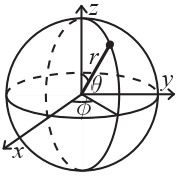
\includegraphics[width=25mm]{src/mathematics/spherical-coordinates}
\end{center}
\[\begin{array}{cc}
          x = r\sin\theta\cos\phi & r = \sqrt{x^2+y^2+z^2}                       \\
          y = r\sin\theta\sin\phi & \theta = \textrm{acos}(z/\sqrt{x^2+y^2+z^2}) \\
          z = r\cos\theta         & \phi = \textrm{atan2}(y,x)
     \end{array}\]

\section{Derivatives/Integrals}
\begin{align*}
     \dfrac{d}{dx}\arcsin x = \dfrac{1}{\sqrt{1-x^2}}  &  &  & \dfrac{d}{dx}\arccos x = -\dfrac{1}{\sqrt{1-x^2}} \\
     \dfrac{d}{dx}\tan x = 1+\tan^2 x                  &  &  & \dfrac{d}{dx}\arctan x = \dfrac{1}{1+x^2}         \\
     \int\tan ax = -\dfrac{\ln|\cos ax|}{a}            &  &  & \int x\sin ax = \dfrac{\sin ax-ax \cos ax}{a^2}   \\
     \int e^{-x^2} = \frac{\sqrt \pi}{2} \text{erf}(x) &  &  & \int xe^{ax}dx = \frac{e^{ax}}{a^2}(ax-1)
\end{align*}

Integration by parts:
\[\int_a^bf(x)g(x)dx = [F(x)g(x)]_a^b-\int_a^bF(x)g'(x)dx\]

\section{Sums}
\begingroup
\allowdisplaybreaks
\begin{flalign}
      & \sum_{i=m}^{n} c^i                         = \frac{c^{n+1} - c^m}{c-1}, c \neq 1                   &  & \\
      & \sum_{i=0}^{n} \binom{n}{i} a^{n-i} b^i    = (a+b)^n                                               &  & \\
      & \sum_{i=0}^{n} \binom{n}{i}                = 2^n                                                   &  & \\
      & \sum_{i=0}^{n} \binom{i}{k}                = \binom{n+1}{k+1}                                      &  & \\
      & \sum_{i=0}^{n} i \binom{n}{i}              = n 2^{n-1}                                             &  & \\
      & \sum_{i=0}^{n} \frac{\binom{n}{i}}{i+1}    = \frac{2^{n+1} - 1}{n+1}                               &  & \\
      & \sum_{i=0}^{n} i! \binom{n}{i}             = \left\lfloor n! \cdot e \right\rfloor                 &  & \\
      & \sum_{i=0}^{n} {}_i P_k \binom{n}{i}       = {}_n P_k (2^{n-k})                                    &  & \\
      & \sum_{i=0}^{n} i \cdot i!                  = (n+1)! - 1                                            &  & \\
      & \sum_{k=0}^{m} \binom{n+k}{n}              = \binom{n+m+1}{n+1}                                    &  & \\
      & \sum_{i=0}^{n} \binom{n}{i}^2              = \binom{2n}{n}                                         &  & \\
      & \sum_{i=0}^{n} \frac{1}{i!}                = \frac{\left\lfloor n! \cdot e \right\rfloor}{n!}      &  & \\
      & \sum_{i=0}^{n} i P_k \binom{n}{i} = P_k (2^{n-k})                                                  &  & \\
      & \sum_{i=1}^{n} i + k P_{k+1} = \sum_{i=1}^{n} \prod_{j=0}^{k} (i+j) = \frac{(n+k+1)!}{(n-1)!(k+2)} &  & \\
      & \sum_{i=0}^{n} i! \cdot \binom{n}{i} = \sum_{i=0}^{n} P_{n}{i} = \lfloor n! \cdot e \rfloor        &  &
\end{flalign}
\endgroup

\section{Series}
$$e^x = 1+x+\frac{x^2}{2!}+\frac{x^3}{3!}+\dots,\,(-\infty<x<\infty)$$
$$\ln(1+x) = x-\frac{x^2}{2}+\frac{x^3}{3}-\frac{x^4}{4}+\dots,\,(-1<x\leq1)$$
$$\sqrt{1+x} = 1+\frac{x}{2}-\frac{x^2}{8}+\frac{2x^3}{32}-\frac{5x^4}{128}+\dots,\,(-1\leq x\leq1)$$
$$\sin x = x-\frac{x^3}{3!}+\frac{x^5}{5!}-\frac{x^7}{7!}+\dots,\,(-\infty<x<\infty)$$
$$\cos x = 1-\frac{x^2}{2!}+\frac{x^4}{4!}-\frac{x^6}{6!}+\dots,\,(-\infty<x<\infty)$$

\section{Probability theory}
Let $X$ be a discrete random variable with probability $p_X(x)$ of assuming the
value $x$. It will then have an expected value (mean)
$\mu=\mathbb{E}(X)=\sum_xxp_X(x)$ and variance
$\sigma^2=V(X)=\mathbb{E}(X^2)-(\mathbb{E}(X))^2=\sum_x(x-\mathbb{E}(X))^2p_X(x)$
where $\sigma$ is the standard deviation. If $X$ is instead continuous it will
have a probability density function $f_X(x)$ and the sums above will instead be
integrals with $p_X(x)$ replaced by $f_X(x)$.

Expectation is linear:
\[\mathbb{E}(aX+bY) = a\mathbb{E}(X)+b\mathbb{E}(Y)\]
For independent $X$ and $Y$, \[V(aX+bY) = a^2V(X)+b^2V(Y).\]

\subsection{Discrete distributions}

\subsubsection{Binomial distribution}
The number of successes in $n$ independent yes/no experiments, each which
yields success with probability $p$ is $\textrm{Bin}(n,p),\,n=1,2,\dots,\,
     0\leq p\leq1$.
\[p(k)=\binom{n}{k}p^k(1-p)^{n-k}\]
\[\mu = np,\,\sigma^2=np(1-p)\]
$\textrm{Bin}(n,p)$ is approximately $\textrm{Po}(np)$ for small $p$.

\subsubsection{First success distribution}
The number of trials needed to get the first success in independent yes/no
experiments, each which yields success with probability $p$ is
$\textrm{Fs}(p),\,0\leq p\leq1$.
\[p(k)=p(1-p)^{k-1},\,k=1,2,\dots\]
\[\mu = \frac1p,\,\sigma^2=\frac{1-p}{p^2}\]

\subsubsection{Poisson distribution}
The number of events occurring in a fixed period of time $t$ if these events
occur with a known average rate $\kappa$ and independently of the time since
the last event is $\textrm{Po}(\lambda),\,\lambda=t\kappa$.
\[p(k)=e^{-\lambda}\frac{\lambda^k}{k!}, k=0,1,2,\dots\]
\[\mu=\lambda,\,\sigma^2=\lambda\]

\subsection{Continuous distributions}

\subsubsection{Uniform distribution}
If the probability density function is constant between $a$ and $b$ and 0
elsewhere it is $\textrm{U}(a,b),\,a<b$.
\[f(x) = \left\{
     \begin{array}{cl}
          \frac{1}{b-a} & a<x<b              \\
          0             & \textrm{otherwise}
     \end{array}\right.\]
\[\mu=\frac{a+b}{2},\,\sigma^2=\frac{(b-a)^2}{12}\]

\subsubsection{Exponential distribution}
The time between events in a Poisson process is
$\textrm{Exp}(\lambda),\,\lambda>0$.
\[f(x) = \left\{
     \begin{array}{cl}
          \lambda e^{-\lambda x} & x\geq0 \\
          0                      & x<0
     \end{array}\right.\]
\[\mu=\frac{1}{\lambda},\,\sigma^2=\frac{1}{\lambda^2}\]

\subsubsection{Normal distribution}
Most real random values with mean $\mu$ and variance $\sigma^2$ are well
described by $\mathcal{N}(\mu,\sigma^2),\,\sigma>0$.
\[ f(x) = \frac{1}{\sqrt{2\pi\sigma^2}}e^{-\frac{(x-\mu)^2}{2\sigma^2}} \]
If $X_1 \sim \mathcal{N}(\mu_1,\sigma_1^2)$ and $X_2 \sim
     \mathcal{N}(\mu_2,\sigma_2^2)$ then
\[ aX_1 + bX_2 + c \sim \mathcal{N}(\mu_1+\mu_2+c,a^2\sigma_1^2+b^2\sigma_2^2) \]

\section{Markov chains}
A \emph{Markov chain} is a discrete random process with the property that the
next state depends only on the current state. Let $X_1,X_2,\ldots$ be a
sequence of random variables generated by the Markov process. Then there is a
transition matrix $\mathbf{P} = (p_{ij})$, with $p_{ij} = \Pr(X_n = i | X_{n-1}
     = j)$, and $\mathbf{p}^{(n)} = \mathbf P^n \mathbf p^{(0)}$ is the probability
distribution for $X_n$ (i.e., $p^{(n)}_i = \Pr(X_n = i)$), where
$\mathbf{p}^{(0)}$ is the initial distribution.

\subsubsection{Stationary distribution}
$\mathbf{\pi}$ is a stationary distribution if $\mathbf{\pi} = \mathbf{\pi P}$.
If the Markov chain is \emph{irreducible} (it is possible to get to any state from any state),
then $\pi_i = \frac{1}{\mathbb{E}(T_i)}$ where $\mathbb{E}(T_i)$  is the expected time between two visits in state $i$.
$\pi_j/\pi_i$ is the expected number of visits in state $j$ between two visits in state $i$.

For a connected, undirected and non-bipartite graph, where the transition
probability is uniform among all neighbors, $\pi_i$ is proportional to node
$i$'s degree.

\subsubsection{Ergodicity}
A Markov chain is \emph{ergodic} if the asymptotic distribution is independent
of the initial distribution. A finite Markov chain is ergodic iff it is
irreducible and \emph{aperiodic} (i.e., the gcd of cycle lengths is 1).
$\lim_{k\rightarrow\infty}\mathbf{P}^k = \mathbf{1}\pi$.

\subsubsection{Absorption}
A Markov chain is an A-chain if the states can be partitioned into two sets
$\mathbf{A}$ and $\mathbf{G}$, such that all states in $\mathbf{A}$ are
absorbing ($p_{ii}=1$), and all states in $\mathbf{G}$ leads to an absorbing
state in $\mathbf{A}$. The probability for absorption in state
$i\in\mathbf{A}$, when the initial state is $j$, is $a_{ij} =
     p_{ij}+\sum_{k\in\mathbf{G}} a_{ik}p_{kj}$. The expected time until absorption,
when the initial state is $i$, is $t_i = 1+\sum_{k\in\mathbf{G}}p_{ki}t_k$.

\pausecol
\addcontentsline{toc}{subsection}{ Distribution table }
\begin{center}
     \renewcommand{\arraystretch}{2.2}
     \begin{tabular}{cccccc}
          \textbf{Distribution} & \textbf{PMF/PDF and Support} & \textbf{Expected Value} & \textbf{Variance} & \textbf{MGF} \\
          \hline
          \shortstack{Bernoulli                                                                                             \\ \Bern($p$)} & \shortstack{$P(X=1) = p$ \\$ P(X=0) = q=1-p$} & $p$ & $pq$ & $q + pe^t$ \\
          \hline
          \shortstack{Binomial                                                                                              \\ \Bin($n, p$)} & \shortstack{$P(X=k) = {n \choose k}p^k q^{n-k}$  \\ $k \in \{0, 1, 2, \dots n\}$}& $np$ & $npq$ & $(q + pe^t)^n$ \\
          \hline
          \shortstack{Geometric                                                                                             \\ \Geom($p$)} & \shortstack{$P(X=k) = q^kp$  \\ $k \in \{$0, 1, 2, \dots $\}$}& $q/p$ & $q/p^2$ & $\frac{p}{1-qe^t}, \, qe^t < 1$\\
          \hline
          \shortstack{Negative Binomial                                                                                     \\ \NBin($r, p$)} & \shortstack{$P(X=n) = {r + n - 1 \choose r -1}p^rq^n$ \\ $n \in \{$0, 1, 2, \dots $\}$} & $rq/p$ & $rq/p^2$ &  $(\frac{p}{1-qe^t})^r, \, qe^t < 1$\\
          \hline
          \shortstack{Hypergeometric                                                                                        \\ \Hypergeometric($w, b, n$)} & \shortstack{$P(X=k) = \sfrac{{w \choose k}{b \choose n-k}}{{w + b \choose n}}$ \\ $k \in \{0, 1, 2, \dots,  n\}$} & $\mu = \frac{nw}{b+w}$ &$\left(\frac{w+b-n}{w+b-1} \right) n\frac{\mu}{n}(1 - \frac{\mu}{n})$& messy  \\
          \hline
          \shortstack{Poisson                                                                                               \\ \Pois($\lambda$)} & \shortstack{$P(X=k) = \frac{e^{-\lambda}\lambda^k}{k!}$ \\ $k \in \{$0, 1, 2, \dots $\}$} & $\lambda$ & $\lambda$ & $e^{\lambda(e^t-1)}$ \\
          \hline
          \hline
          \shortstack{Uniform                                                                                               \\ \Unif($a, b$)} & \shortstack{$ f(x) = \frac{1}{b-a}$ \\$ x \in (a, b) $} & $\frac{a+b}{2}$ & $\frac{(b-a)^2}{12}$ &  $\frac{e^{tb}-e^{ta}}{t(b-a)}$\\
          \hline
          \shortstack{Normal                                                                                                \\ $\N(\mu, \sigma^2)$} & \shortstack{$f(x) = \frac{1}{\sigma \sqrt{2\pi}} e^{-\sfrac{(x - \mu)^2}{(2 \sigma^2)}}$ \\ $x \in (-\infty, \infty)$} & $\mu$  & $\sigma^2$ & $e^{t\mu + \frac{\sigma^2t^2}{2}}$\\
          \hline
          \shortstack{Exponential                                                                                           \\ $\Expo(\lambda)$} & \shortstack{$f(x) = \lambda e^{-\lambda x}$\\$ x \in (0, \infty)$} & $\frac{1}{\lambda}$  & $\frac{1}{\lambda^2}$ & $\frac{\lambda}{\lambda - t}, \, t < \lambda$\\
          \hline
          \shortstack{Gamma                                                                                                 \\ $\Gam(a, \lambda)$} & \shortstack{$f(x) = \frac{1}{\Gamma(a)}(\lambda x)^ae^{-\lambda x}\frac{1}{x}$\\$ x \in (0, \infty)$} & $\frac{a}{\lambda}$  & $\frac{a}{\lambda^2}$ & $\left(\frac{\lambda}{\lambda - t}\right)^a, \, t < \lambda$\\
          \hline
          \shortstack{Beta                                                                                                  \\ \Beta($a, b$)} & \shortstack{$f(x) = \frac{\Gamma(a+b)}{\Gamma(a)\Gamma(b)}x^{a-1}(1-x)^{b-1}$\\$x \in (0, 1) $} & $\mu = \frac{a}{a + b}$  & $\frac{\mu(1-\mu)}{(a + b + 1)}$ & messy \\
          \hline
          \shortstack{Log-Normal                                                                                            \\ $\mathcal{LN}(\mu,\sigma^2)$} & \shortstack{$\frac{1}{x\sigma \sqrt{2\pi}}e^{-(\log x - \mu)^2/(2\sigma^2)}$\\$x \in (0, \infty)$} & $\theta = e^{ \mu + \sigma^2/2}$ & $\theta^2 (e^{\sigma^2} - 1)$ & doesn't exist\\
          \hline
          \shortstack{Chi-Square                                                                                            \\ $\chi_n^2$} & \shortstack{$\frac{1}{2^{n/2}\Gamma(n/2)}x^{n/2 - 1}e^{-x/2}$\\$x \in (0, \infty) $} & $n$  & $2n$ & $(1 - 2t)^{-n/2}, \, t < 1/2$\\
          \hline
          \shortstack{Student-$t$                                                                                           \\ $t_n$} & \shortstack{$\frac{\Gamma((n+1)/2)}{\sqrt{n\pi} \Gamma(n/2)} (1+x^2/n)^{-(n+1)/2}$\\$x \in (-\infty, \infty)$} & $0$ if $n>1$ & $\frac{n}{n-2}$ if $n>2$ & doesn't exist\\
          \hline
     \end{tabular}
\end{center}
\clearpage
\resumecol
\chapter{ Strings }

\section{ Hashing }
\importcode{code/strings/Hashing.h}

\section{ KMP }
\importcode{code/strings/KMP.h}

\section{ Manacher }
\importcode{code/strings/Manacher.h}

\section{Miscalenous}
\section{Optimization Tricks}

\subsection{Bit Hacks}
\begin{itemize}
    \item \( x \& -x \) gives the least significant bit in \( x \).
    \item Use \inlinecode!for (int x = m; x;) { --x &= m; }! to loop over all subset
          masks of \( m \) (except \( m \) itself).
    \item To find the next number after \( x \) with the same number of bits set, use:
          \inlinecode!c = x &-x, r = x + c; (((r^x) >> 2) / c) | r!
    \item For cumulative sums of subsets, use:
          \begin{codesnippet}
    for (int b=0; b < k; i++)
        for (int i=0; i < (1<<k); i++) 
            if (i&1<<b) D[i] += D[i ^ (1<<b)]; 
          \end{codesnippet}
\end{itemize}

\subsection{Pragmas}
\begin{itemize}
    \item Use \inlinecode!#pragma GCC optimize ("Ofast")! to enable GCC's
          auto-vectorization and better optimization for floating points (assumes
          associativity and turns off denormals).
    \item Use \inlinecode!#pragma GCC target ("avx,avx2")! to potentially double
          performance of vectorized code, though it may cause crashes on older machines.
          Consider using \inlinecode!#pragma GCC target ("sse4")! for older
          architectures.
    \item Use \inlinecode!#pragma GCC optimize ("trapv")! to kill the program on integer
          overflows (but it may slow down execution).
\end{itemize}
    % This line includes the content file, where topics and articles will be defined

\end{multicols*}

\end{document}
